\chapter{Obecný úvod do architektury mikroslužeb}\label{ch:msa-intro}

\chaptersummary{
   \begin{ul}
      \item obecné informace o architektuře a proč je důležitá,
      \item porovnání vybraných architektur – \g{MSA}, \g{MA} a \g{SOA},
      \item typy dekompozice specifikace na \g{MSA} architekturu,
      \item komunikace mezi mikroslužbami a řešení závislostí,
      \item testování a validace mikroslužeb,
      \item nasazení mikroslužeb na server a základní monitorování,
      \item krátký úvod do služeb na straně webového klienta.
   \end{ul}
}


Softwarovou architekturu jako pojem je těžké exaktně definovat, každý vývojář k ní může přistupovat a vnímat jinak.
Obecně může být popsána jako jistý řád a pravidla, vzniklá následkem mnoha rozhodnutí v průběhu analýzy a vývoje produktu.
Veškerý následující rozvoj by se měl striktně řídit těmito pravidly, aby umožnil vznik dlouhodobě udržovatelného výsledku~\cite{softarch}.

Vývoj softwaru bez architektury nebo s nepřesně definovanou osnovou může být přínosný v krátkodobé perspektivě nebo z hlediska šetření počátečních nákladů na čas a finanční složky~\cite{softarch}.
V případě dlouhodobého projektu to však může znamenat hromadění technického dluhu~\cite{archoworthit}.
Dle článku~\cite{archoworthit} přínos architektury lze vizuálně znázornit grafem~\ref{fig:architecture-line}, kde je uvedena kumulativní funkcionalita v závislosti čase spotřebovaným projektem.
Používání architektury ze začátku způsobuje zpomalení vývoje, ale od jisté hranice výhody se stává přínosnou a urychluje rozvoj.
Tento předpoklad však funguje pouze v případě, že se jedná o dobře zvolenou a popsanou architekturu (v textové nebo diagramové podobě), která má pozitivní vliv a je dostatečně ohebná~\cite{archoworthit}.


\begin{figure}[htbp]
   \centering
   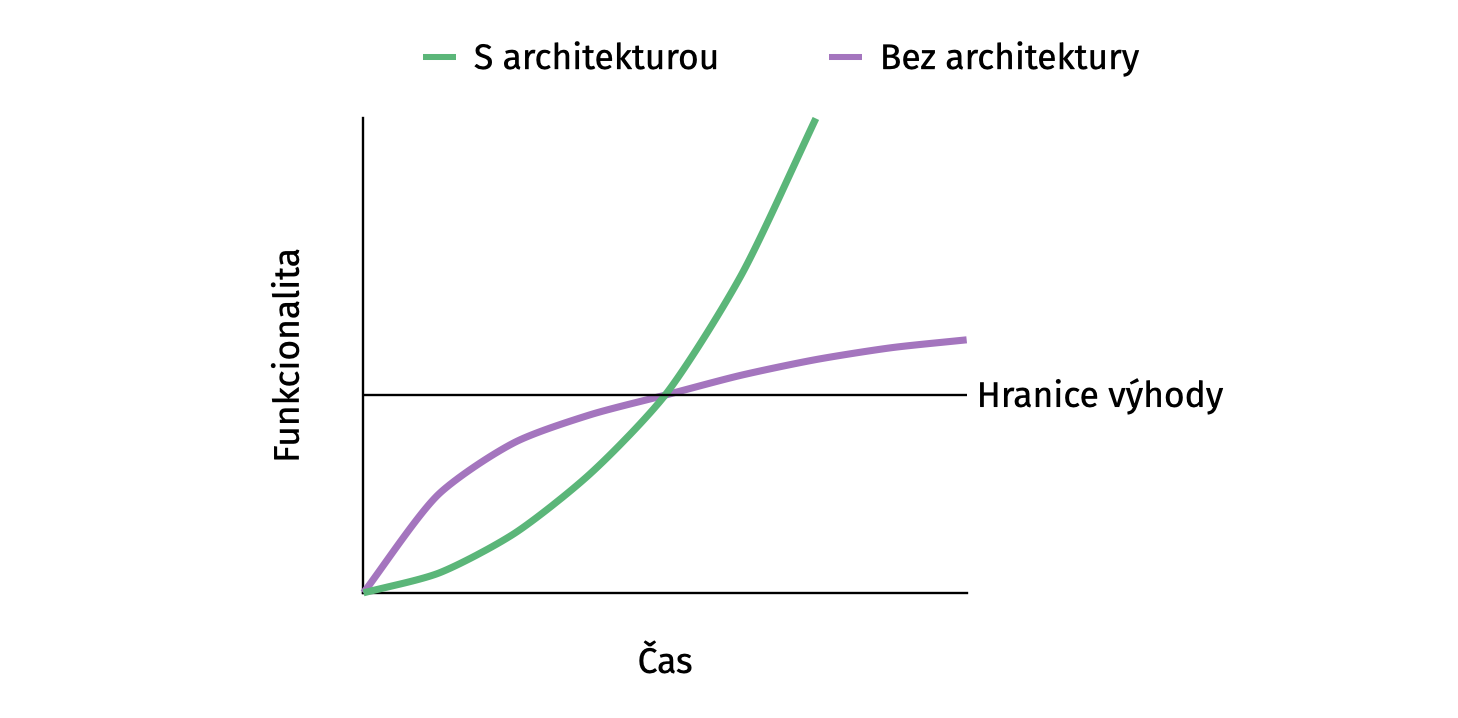
\includegraphics[max width=\textwidth]{assets/architecture-line}
   \caption[Bod přínosu dodržování architektury]{Bod přínosu dodržování architektury~\cite{archoworthit}}\label{fig:architecture-line}
\end{figure}


Ačkoliv neexistuje přesná definice architektury obecně, existují detailněji popsané typy architektur, které jsou vhodné pro vývoj aplikací.
Jejich volba a případná adaptace vyžaduje pochopení konečného cíle požadovaného výsledku~\cite{softarch}.
V návaznosti na zadání diplomové práce v dané kapitole bude popisována především \g{MSA} a bude porovnávána s jinými architekturami, které by ji potenciálně mohly nahradit.
Tyto vybrané architektury – \g{MA}, \g{SOA}\footnote{též architektura orientovaná na služby}, \g{SA} – budou zkoumány vzhledem k přístupu k určitým aspektům, poskytovaným možnostem a výhodám a nevýhodám vůči \g{MSA}.
Vzhledem k dříve použitému jazyku TypeScript/JavaScript budou i srovnání zaměřeno na tento jazyk, případně Node.js prostředí.


Než se začne s konkrétním porovnáním, je třeba definovat jeden společný pojem všech 3 architektur – službu.
Služba v této práci je chápána jako atomicky fungující celek, z~větší části nezávislý na ostatních – soustředí se na konkrétní funkcionalitě (nebo skupině funkcionalit), má přístup k databázovému úložišti a veškerá komunikace probíhá přes striktně definované rozhraní (vizualizaci takové služby je možné vidět na~obrázku~\ref{fig:service-abstract}).
Může fungovat jako celek poskytující, přijímající a zpracovávající nebo předávající datové zprávy.
Jakýkoliv jiný vliv, než přes dohodnuté rozhraní, je ignorován a musí být ideálně eliminován.
Rozhraní takové služby může být popsáno s pomocí samostatné dokumentace nebo dokumentovaného kódu.


\begin{figure}[htbp]
   \centering
   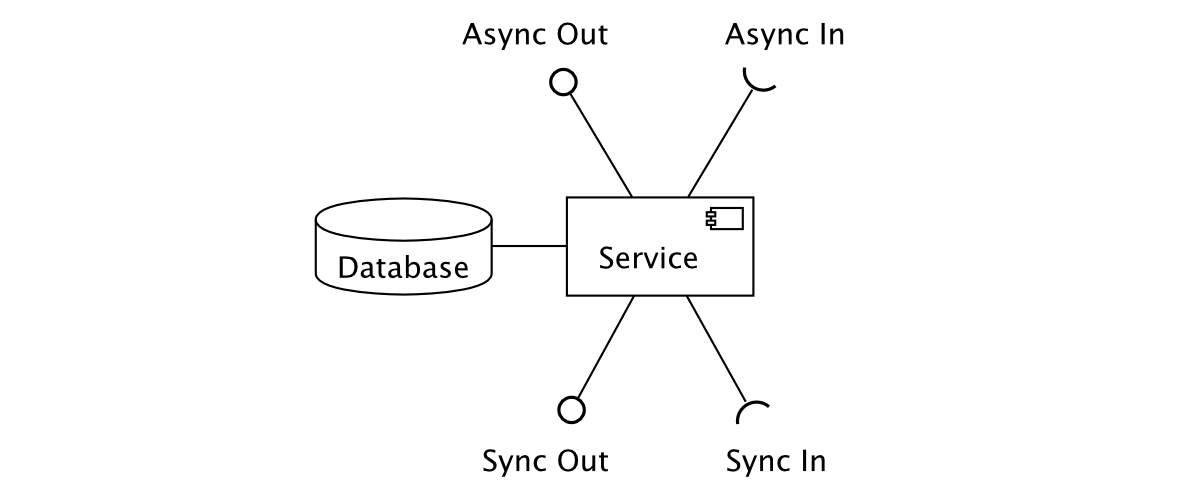
\includegraphics[max width=\textwidth]{assets/service}
   \caption{Abstraktní znázornění služby}\label{fig:service-abstract}
\end{figure}


Kvůli nejednoznačnosti pojmu \enquote{architektura} nejspíš existuje nespočetné množství modifikací a adaptací výše uvedených architektur (\g{MA}, \g{SOA}, \g{MSA}, \g{SA}), proto se bude předpokládat, že se jedná o takto definované instance:

\begin{dl}
   \item[\g{MA}] – jednoprocesový program atomické povahy – nelze z něho jednoduše vyčlenit funkční celky, které by se daly beze změn využívat v jiných programech.
   Obsahuje globální jednorázové připojení k datovému zdroji, které se provádí během startu.
   Takový program je sám o sobě službou.
   \item[\g{SOA}] – jednoprocesový program s interním rozdělením na služby, které mezi sebou komunikují s pomocí zpráv přímo s využitím vyčleněného rozhraní nebo přes \g{ESB} – sběrnicí určenou pro centralizaci komunikace mezi službami.
   Vazba na datový zdroje může, ale nemusí být jedna (každá služba může mít samostatné připojení).
   \item[\g{MSA}] – několikaprocesový systém služeb (každá služba má právě jeden proces) organizovaný do větší interně kompatibilní struktury.
   \item[\g{SA}] – architektura aplikace, která postrádá kontinuálně běžící serverový proces a je pouze rozmístěna na \g{FaaS} řešení.
   Jinými slovy funkcionalita není spuštěna v nepřerušovaném prostředí (jako démon), ale je dostupná na požádání.
   Během uživatelského dotazu je vytvořena potřebná instance aplikace, případně navázáno databázové spojení, vykonán požadavek a následně je instance odstraněna.
\end{dl}

\newpage



Softwarová architektura jako pojem není přesně definována \cite{softarch}

Arichitektura může být popsána jako jistý řád a pravidla, dle kterých je celá aplikace postavena.
Existují nějaké šablony architektury, které jsou vhodné pro vývoj aplikací


V dané kapitole bude popisována především \gls{MSA} a bude porovnávana s jinými architekturami, které by ji potenciálně mohly nahradit.
Tyto vybrané architektury – \gls{MA}, \gls{SOA}\footnote{též architektura orientovaná na služby}, \gls{SA} – budou zkoumány vzhledem k přístupu k určitým aspektům, poskytovaným možnostem a výhodám a nevýhodám vůči \gls{MSA}.



Služba (bez vazby na architekturu) je chápána jako atomicky fungující celek, z větší části nezávislý na ostatních – soutředí se na konkrtétní funkcionalitu, má vlastní databázi (nebo schéma) s výhradným přístupem a veškerá komunikace probíhá přes striktně definované rozhraní.
Jakýkoliv jiný vliv, než přes dohodnuté rozhraní, musí být eliminován.

Jelikož existuje nespočetné množství modifikací výše uvedených architektur, bude se předpokládat, že se jedná o takto definované instance:


%https://www.ibm.com/cloud/learn/soa#toc-soa-vs-mic-BjTfju28

\begin{dl}
   \item[\gls{MA}] – jednoprocesový program atomické povahy – nelze z něho jednoduše vyčlenit funkční celky, které by se daly beze změn využívat v jiných programech.
   Obsahuje globální jednorázové připojení k databázi, které se provádí během startu programu a kontroluje aktuální stav migrací (případně vykonává chybějící).
   \item[\gls{SOA}] – jednoprocesový program s interním rozdělením založeným na \gls{ESB} – sběrnicí určenou pro centralizaci komunikace mezi službami.
   Jednotlivé služby tvoří samostatně fungující moduly, jež veškerou komunikaci provádí skrz přesně definované rozhraní \gls{ESB}.
   Obdobně, jako u \gls{MA} existuje jedno
   \item[\gls{MSA}] –
   \item[\gls{SA}] – architektura aplikace, která postrádá neustále běžící serverový proces a je pouze rozmístěna na \gls{FaaS} řešení.
   Jinými slovy funkcionalita není spuštěna v nepřerušovaném prostředí (jako démon), ale je dostupná na požádání.
   Při dotazu (například REST) je vytvořena potřebná instance aplikace, případně navázáno databázové spojení, vykonán požadavek a následně je instance odstraněna.
   Taková aplikace nemůže být stavová v obvyklém slova smyslu.
   Kvůli průběhu zpracování se rovněž nehodí pro náročné aplikace. \TODO{zdroj}
\end{dl}

Pro porovnání architektur bylo vybráno několik klíčových pojmů, které mohou během návrhem a implementací programu mít nějvětší vliv na rozhodování o výběru architektury.

+- MA OR 29


\begin{dl}
   \item[Datové úložiště] – využití persistentního úložiště (SQL/NoSQL databáze) pro zápis a čtení informací.
   Počáteční inicializace databáze, vytvoření struktury, migrace
\end{dl}
\begin{ul}
   \item \gls{MA} – není náročná pro testování.
   \item \gls{SOA} – rovněž může být testována
   \item \gls{MSA} – plnohodnotné testování celé struktury vyžaduje její nasazení na server.
\end{ul}

\begin{dl}
   \item[Nezávislost] – popis
\end{dl}
\begin{ul}
   \item \gls{MA} – něco umí
   \item \gls{SOA} – něco umí
   \item \gls{MSA} – něco umí
\end{ul}

\begin{dl}
   \item[Radikální změny] – složitost změny nebo přidání business logiky do aplikace, která by měl dopad na větší část dosavadní aplikace.
\end{dl}
\begin{ul}
   \item \gls{MA} –
   Z hlediska datového úložiště bude potřeba dělat pouze jednu migraci
   \item \gls{SOA} – něco umí
   \item \gls{MSA} – něco umí
\end{ul}

\begin{dl}
   \item[Tolerace chyb] – popis
\end{dl}
\begin{ul}
   \item \gls{MA} – něco umí
   \item \gls{SOA} – něco umí
   \item \gls{MSA} – něco umí
\end{ul}

\begin{dl}
   \item[Komunikační latence] – popis
\end{dl}
\begin{ul}
   \item \gls{MA} – něco umí
   \item \gls{SOA} – něco umí
   \item \gls{MSA} – něco umí
\end{ul}

\begin{dl}
   \item[Škálování] – popis
\end{dl}
\begin{ul}
   \item \gls{MA} – něco umí
   \item \gls{SOA} – něco umí
   \item \gls{MSA} – něco umí
\end{ul}

\begin{dl}
   \item[Konzistence] – popis
\end{dl}
\begin{ul}
   \item \gls{MA} – něco umí
   \item \gls{SOA} – něco umí
   \item \gls{MSA} – něco umí
\end{ul}

\begin{dl}
   \item[Nasazení] – popis
\end{dl}
\begin{ul}
   \item \gls{MA} – něco umí
   \item \gls{SOA} – něco umí
   \item \gls{MSA} – něco umí
\end{ul}

\begin{dl}
   \item[Testování] – schopnost psaní automatizovaných testů, které se vyplní při spuštění aplikace.
\end{dl}
\begin{ul}
   \item \gls{MA} – něco umí
   \item \gls{SOA} – něco umí
   \item \gls{MSA} – něco umí
\end{ul}

\section{Využití \g{MSA} pro modelování světa}\label{sec:msa-model-of-world}

Pro člověka nejspíš neexistuje nic přirozenějšího, než prostředí, ve kterém se pohybuje a kterému rozumí – od osobních věcí a proseců, jež musí vykonávat, až po uspořádání světa – město, stát, planeta, politické a sociální vztahy, komunikace s institucemi a interakce s rodinou.

Všechny tyto činnosti můžeme popsat pomocí subjektů – samostatných účastníků procesů, rozhraní, které poskytují pro komunikaci, a zpráv\footnote{Zprávou se rozumí informace poskytnutá v samostatné struktuře – například \g{JSON} nebo \g{XML}}, jež se předávají v rámci komunikace.
Každý subjekt je skupinou izolovaných funkcí s různě kompikovanou sadou komunikačních kanálů.
Může mít svoje potřeby a může vytvářet podněty pro ostatní subjekty.
Ne každý subjekt je schopen zpracovávat veškerou informaci, která k němu přichází od jiných subjektů.

Daný konecept naprosto přesně napodobuje \g{MSA}.
Jednotlivé subjekty jsou mikroslužby, mají vlastní rozhraní a vysílají informace v přesně definovaných strukturách.
Mohou existovat samostatně, i když jejich smysl existence nemusí existovat.
Zároveň jsou schopny zachytit a zpracovat zprávy, které byly určeny pro jejich použití a formát kterých je popsaný ve vnitřní logice.

V případě mírného zjednodušení se můžeme dostat ke konceptu \g{SOA}.
Subjekty zachovávají způsob komunikace s pomocí zpráv, ale již nejsou samostatní, potenciálně fungující celky, nýbrž moduly jednoho většího bloku.
Komunikace u takové architektury může být centrállně řízena \g{ESB}.\cite{soavsmsa}

Monolitní architektura v provonání se \g{SOA} zjednodušuje i samotné rozdělení do modulů.
Stále se jedná o samostatně fungující celek, ale vnitří struktura už postrádá moduly s odděleným rozhraním komunikace s využitím zpráv.
V rámci modelování světa se dá představit jako interně nedělitelný celek, který pouze poskytuje rozhraní pro komunikaci, tudíž je to subjekt a v rámci \g{MSA} může představovat mikroslužbu.

Na základě výše uvedených informací by logicky bylo nejjednodušší vždy vytvářet pouze \g{MSA} architekturu, protože je pro pochopení nejsnažší kvůli zkušenostem z každodenního života.
Každý subjekt má svoje potřeby (potřeva vytvořit zprávu, potřeba zpracovat příchozí právu) a o zbylé aspekty se nestará.
Problém nastává kvůli komplexnosti takového konceptu.
Jakékoliv rozdělení celku implicitně předpokládá nové náklady pro definování komunikace, které jsou náročné pro představu.
Proto může být nejvýhodnější začít architektorou s nejvíc redukovaným rozdělením – monolitem a dle potřeby měnit hloubku rozdělení.

Navíc při detailním zkoumání ve všech výše uvedených architekturách se dá vypozorovat rekurzivita.
Monolitická aplikace nebo \g{SOA} aplikace může tvořit mikroslužbu v rámci \g{MSA}.
\g{MSA} aplikace může tvořit mikroslužbu jiné \g{MSA} a fungovat jako monolit pro ostatní.

\section{Dekompozice na \g{MSA}}\label{sec:msa-decomposition}

Projekt, u něhož bylo rozhodnuto o \g{MSA}, vyžaduje, jako jeden z kroků před implementací, dekompozici zadání na oblasti, dle kterých budou následně vytvářeny jednotlivé služby.
Stejně jako v případě myšlenky modelování světa, účastníky procesů budou subjekty a jejich rozhraní pro komunikaci, které v případě projektu lze vyčíst specifikace.

Jinými slovy definování konkrétní architektury projektu se dá provádět postupně ve 3 fázích~\cite{msachris} \TODO{OR74} (vizualizace na obrázku~\ref{fig:msa-decomposition-flow}):


\begin{ol}
   \item Definování operací zpracovávaných serverem – na základě specifikace projektu, ve které jsou popsány požadavky očekávané od serverové části aplikace, formulujeme do konkrétních volání – získat, vytvořit, aktualizovat data.
   \item Definování možných služeb – pro dekompozici na konkrétní služby existují dva základní přístupy – rozdělení dle subdomén a prozdělení dle obchodních potřeb~\cite{msachris}, oba přístupy budou stručně popsány v dalších podkapitolách.
   Oba přístupy vychází z navrhnutých volání a přiřazuje je jednotlivým službám.
   \item Definování propojení požadavků se službami a komunikace služeb mezi sebou – prohlubuje definovanou komunikaci mezi službami a vytváří konkrétní interní a externí spoje.
\end{ol}


\begin{figure}[htbp]
   \centering
   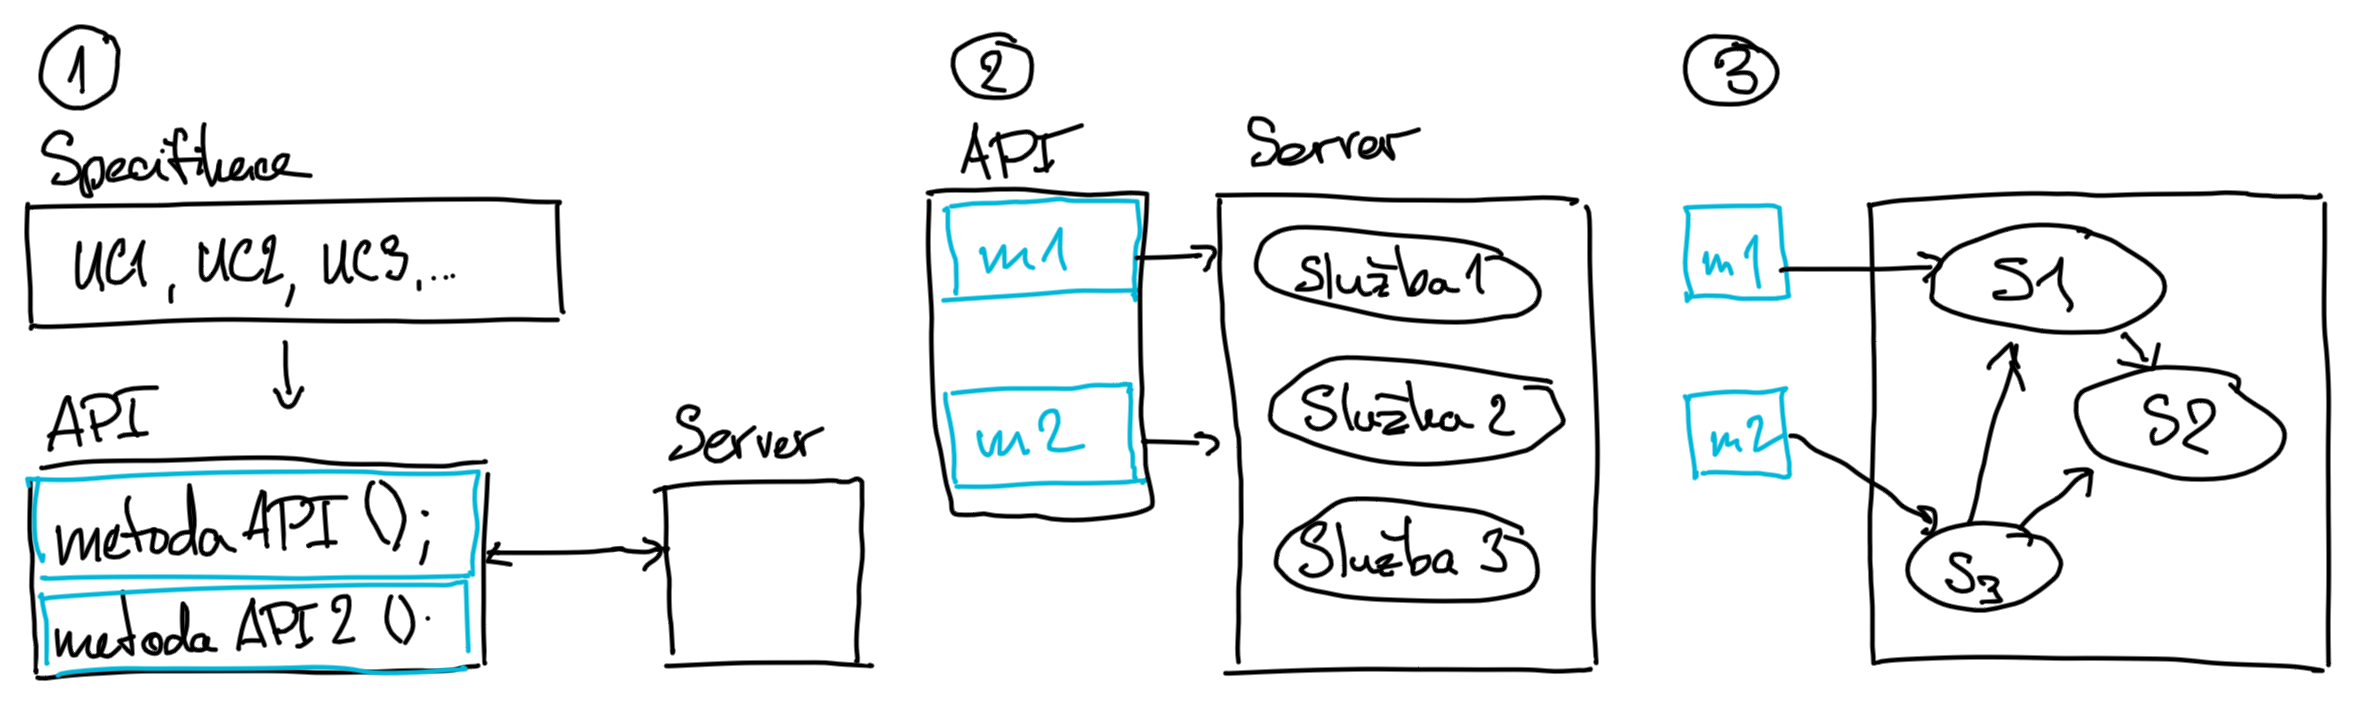
\includegraphics[max width=\textwidth]{assets/draft-decomposition-flow}
   \caption{Tři kroky návrhu \g{MSA}}\label{fig:msa-decomposition-flow}
\end{figure}


V rámci rozdělování operací do konkrétních služeb (stejně jako návrh služeb) mohou pomoci i návrhové vzory týkající se vývoje samotného, jako jsou například:


\begin{dl}
   \item[Princip jedné odpovědnosti] – každá třída musí mít právě jeden důvod, proč se měnit~\cite{srp}.
   V kontextu mikroslužeb se to rovněž vztahuje i na službu samotnou – musí se zabývat pouze jednou subdoménou řešeného problému.
   \item[Vysoká soudržnost] – služba obashuje vše potřebné pro řešení oblasti, za níž je odpovědná~\cite{lchc}.
   \item[Nízká provázanost] – služba může získávat informace z ostatních zdrojů, ale snížená provázanost ulehčuje vývoj~\cite{lchc}.
\end{dl}


Vzhledem k širokému rozsahu dostupných modifikací \g{MSA} je sem možné začlenit mnohem větší spektrum pravidel a doporučení, vždy záleží na aspektech konkrétního zadání.
Některé z nich budou popsány v následujících kapitolách a mohou mít vliv na rozhodnutí spojená s dekompozicí vytvářené funkcionality.



\subsection{Dekompozice dle obchodních potřeb}\label{subsec:msa-decomposition-business}
Dekompozice oblastí dle obchodních potřeb je jednou ze dvou základních možností, jak dokompozici provádět~\cite{msachris}.
Soutředí se na vazbě s architekturou společnosti, neboli něčem, co firmě přináší užitečnou hodnotu~\cite{decompbusiness}.
Uvažujme případ, že o vytvoření \g{MSA} požádala firma, která zpracovává různé druhý objednávek - oblečení, potraviny, sportovní nářadí a spravuje interní pracovníky – stálé zaměstnance a příležitostnou výpomoc.
Z takové struktury by mohlo vzniknout 5 služeb, které by spravovaly:


\begin{ul}
   \item objednávky oblečení,
   \item objednávky potravin,
   \item objednávky sportovního nářadí,
   \item správu zaměstnanců,
   \item správu výpomoci.
\end{ul}



\subsection{Dekompozice dle subdomén}\label{subsec:msa-decomposition-domain}
Dekompozice z hlediska subdomény, která představuje druhý způsob rozdělení, na rozdíl od obchodních požadavků nevnímá architekturu společnosti jako zásadní, i když je nutná, a upřednostňuje logické rozdělování~\cite{decompsubdomain}.
V případě stejného příkladu firmy by dekompozice dle subdomén mohla vypadat následovně:


\begin{ul}
   \item objednávky,
   \item správa pracovníků.
\end{ul}


Takové služby už by nebyly specializované na konkrétním užití a tudíž by mohly být větší nároky na jejich schopnost se přizpůsobovat potřebám \g{IS}.

Typ dekompozice nelze přesně stanovit, je třeba se dívat na všechny potřebné aspekty zkoumané domény a přizpůsobovat dané metody konkrétním situacím~\cite{msachris}.


\section{Závislosti a komunikace}

Mikroservisy jsou vždy nezávislé z hlediska procesů, ale musí udržovat kompatibilní \g{API} s ostatním prostředím.
Takové závislosti se nejlépe kontrolují verzováním jednotlivých mikroservis s pomocí sématického verzování.
Zde je třeba najít konkrétní nástroj pro tuto kontrolu.


- Orchestrace VS Choreografie

\subsection{Komunikace}
- sync/async
- latence
- problém řetězových závislotí


\section{Testování a automatizace}

Daná kapitola se věnuje problematice automatizace testování projektu napsaného v architektuře mikroslužeb s dodaným uživatelským webovým rozhraním.
V rámci testování budeme uvažovat pouze následující kategorie:

\begin{dl}
   \item[Jednotkové testování] – testování nejmenších částí implementace (funkce, třídy aj.),
   \item[Integrační testování] – testování integrací v rámci jedné \g{MS} i mezi \g{MS},
   \item[Funkční testování] – testování funkčnosti bez znalosti interní implementace~\cite{testtypes} dle testovacích scénářů,
   \item[Testování výkonu] – testování systému v předem dané zátěži.
   \item[Testování spolehlivosti] – testování způsobu chování v případech přetížení/výpadku a schopnost se obnovit po výpadku~\cite{testtypes2}.
\end{dl}

V ideálním případě je snaha mít každý automatizovaný typ testování automaticky spouštěný ve správnou chvíli během vývojového cyklu a nasazení sytému.
V případě neexistence možnosti vytvořit automatizaci nebo automacké spouštění, bude potřebný typ testování
Akceptovaným bude rovněž dokumentace s


Existují i další typy testů, jež se mohou automatizovat – testy bezpečnosti, kompatibility, přenositelnosti apod.
V dané práci se jimi zabývat nebude.


\section{Nasazování}\label{sec:msa-deployment}

Nasazení mikroslužeb je jedna ze závěrečných fází vývoje systému, pokrývá široké spektrum možností – rozmístění produkčních balíčků na samostatných fyzických serverech, cloud-řešení, v klasterech, s vyvažováním zátěže, replikací apod.
Daná podkapitola se bude věnovat pouze společným rysům – přípravě pro všechny typy nasazení – a kontejnerizací, jež je vyžadována zadáním diplomové práce.


\subsection{Správa zdrojového kódu}\label{subsec:msa-deployment-code}

Služba, případně mikroslužba, z hlediska chování byla v této práci definována jako samostatný, atomicky fungující celek.
Toto se týká i existence spuštěné instance – musí být schopna existovat samostatně (alespoň z hlediska propojení s ostatními službami).
Taková vlastnost má důležitý dopad na potřebné horizontální škálování a rozložení zátěže v nejvyužívanějších částech systému~\cite{monomulti}.

I přes takové předpoklady samotnou správu zdrojového kódu je možné uspořádat jak do jednoho (monorepozitář) tak i více repozitářů (za předpokladu, že se využívá \g{VCS} git).
Oba přístupy mají své výhody a nevýhody.


\begin{dl}
   \item[Monorepozitář] – existence jednoho repozitáře, kde jednotlivé služby jsou umístěny do vlastních složek.

   \textbf{Výhody}
   \begin{ul}
      \item Celý produkt je uchováván na jednom místě - pro tým to může znamenat lepší podmínky pro testování a vývoj, jelikož mají dostupné všechny vyvíjené častí všemi týmy~\cite{monomulti}.
      \item V případě refaktorování nebo testování systému je možné vše provádět na~jednom místě~\cite{monomulti}.
      \item Vývojové prostředí je možné nastavit tak, že všechny služby budou sdílet stejnou konfiguraci (kontrola kvality kódu, formátování a další)~\cite{monomulti}.
   \end{ul}

   \textbf{Nevýhody}
   \begin{ul}
      \item Obrovské množství služeb v jednom repozitáři může znepřehlednit vývoj – git historie se týká nejen jednoho produktu, ale všech – značky a větve budou sdílené pro všechny služby.
      \item Existence možného zásahu do zdrojového kódu služeb vývojáři, jež pro to nemají formální oprávnění~\cite{monomulti}.
   \end{ul}

   \item[Více repozitářů] – každá služba má vlastní repozitář, který je naprosto soběstačný.

   \textbf{Výhody}
   \begin{ul}
      \item Přesné rozdělení vývojových částí a přístupů mezi jednotlivými vývojovými týmy~\cite{monomulti}.
      \item Přehledná git historie pro každou službu včetně značek.
   \end{ul}

   \textbf{Nevýhody}
   \begin{ul}
      \item Absence jednoduchého spuštění všech částí projektu~\cite{monomulti}.
      \item V případě existence sdílených zdrojových kódů, je nutné tuto situaci řešit jinými způsoby, než extraci do sdíleného prostoru nadsložek.
   \end{ul}
\end{dl}


Ze subjektivní zkušenosti je do tohoto přehledu možné přidat ještě jeden způsob vedení projektu.
Spočívá v kombinaci obou přístupů s využitím \h{git submodules}.
V~takovém případě struktura projektu je organizována následovně:

\begin{ul}
   \item Každá služba má svůj vlastní repozitář a jejich vývoj je nezávislý.
   \item Existuje jeden repozitář, který importuje všechny služby jako git submoduly a přidává vhodnou konfiguraci vně submodulů (například \h{docker-compose}, testy apod.).
\end{ul}

Takový přístup přináší některé výhody monorepozitáře, ale přístup k jednotlivým službám je samostatný a může být omezován právy pro každý repozitář.
Tzn.
v případě snahy o jednotnou statickou analýzu kódu (či obdobné záležitosti) je možné přesunou konfigurace ze všech repozitářů mikroslužeb do společného repozitáře se submoduly a odkázat původní konfigurace na konfiguraci v nadsložce.
Tímto zásahem se ale znemožní separátní vývoj a bude potřeba vždy stahovat hlavní repozitář a z toho submodul, nad kterým se má provádět vývoj.



\subsection{Kontejnerizace}\label{subsec:msa-deployment-containerization}
Kontejnerizace je jistý způsob virtualizace za použitím menšího množství systémových zdrojů, než u plnohodnotné virtualizace~\cite{kontejnerizace}.
Základní myšlenka spočívá v přípravě soběstačného balíčku (obrazu) s programem, který by se dal spouštět jednoduchým vytvářením nové instance (kontejneru) v jakémkoliv prostředí, které poskytuje dostatečné základní rozhraní~\cite{dockercontainer}.

V případě JavaScript aplikací založených na Node.js prostředí a využitím služby Docker se bude jednat o následující proces:

\begin{dl}
   \item [Stažení výchozího prostředí] – obraz prostředí, ze kterého bude mikroslužba vycházet, v tomto případě \h{node}.
   \item [Přidání npm/yarn závislostí] – do obrazu jsou staženy všechny vnější závislosti.
   \item [Přidání a sestavení samotného projektu] – do obrazu jsou přidány zdrojové soubory samotného programu a spuštěno sestavení.
   \item [Otevření potřebných komunikačních kanálů] – mikroslužba komunikuje na vlastním, předem určeném portu.
   Po vytvoření instance tento port musí být otevřen pro~komunikaci s kontejnerem.
   \item [Definování příkazu pro spuštění] – definice sekvence příkazů, které během vytvoření kontejneru připraví a spouští příkaz pro start webového serveru.
\end{dl}

Takto se musí připravit každá služba v rámci systému.
Spuštění celého projektu následně může být řízeno \h{docker-compose}, který kromě definovaných mikroslužeb ještě poskytne databáze a další potřebné programy třetích stran.

\section{Monitorování}\label{sec:msa-monitoring}

Monitorování je důležitou součástí vývoje a přizpůsobování mikroslužeb a aplikací obecně.
Dává přehled o stavu sytému a může napomáhat predikci například budoucí zátěže na základě historických dat.
Sledované hodnoty můžeme rozdělit na tři hlavní skupiny~\cite{msactions}:

\begin{dl}
   \item [Metriky] – měřitelné hodnoty latence, chyb, zátěže a saturace systému.
   Může se jednat například o počet požadavků na server, počet chyb, objemu předaných dat, pokusů o opakované zpracování informací, využitou paměť a další hodnoty~\cite{msactions}.
   Takové historické informace se následně mohou podílet na přizpůsobování sytému dle nároků a potřeb.
   \item [Logy] – informace o uskutečněných událostech.
   \item [Stopy] – detailní záznamy o chybách a jejich původu.
\end{dl}

Na takovém rozdělení se zakládá například i populární~\cite{grafanapop} platforma pro vizualizaci metrik Grafana~\cite{grafana}.

Monitorování v architektuře mikroslužeb je samostatná oblast s mnoha způsoby realizace, analýzy a zpracování.
Vzhledem k širokému rozsahu nebude blíže zkoumána, až na návrhový vzor \h{Health Check}.


\subsection{Health check}\label{subsec:msa-monitoring-healthcheck}

Vzor \h{Health Check} je jednoduchým nástrojem pro monitorování aktuálního stavu mikroslužby~\cite{healthcheck}.
Jedná se o speciální \g{API} \h{GET} rozhraní, které poskytuje základní informace o stavu mikroslužby.
Může se jednat například o název, verzi, stavu komunikce, stavu fyzického zařízení a další informace~\cite{healthcheck}.

Takové rozhraní, i když poskytuje jednoduchou kontrolu, tak nese i nevýhodu v podobě nedostupnosti, pokud celá mikroslužba nefunguje.

\section{Klientská část}\label{sec:testing-client-app}

Na straně klinsta se bude provádět testování

\subsection{Jednotkové testy}\label{subsec:testing-client-app-unit}

Obdobně, jako v případě každé \g{MS} pro jednotlivé části implementace byly napsány jednotkové testy, které se prováděly buď manuálně, nebo automaticky (vynuceně) během každé \enquote{push} akce v \h{git}.
Vynucená kontrola byla řešena s pomocí \h{git} hooks.

Následně byla automatizována kontrola základních interakcí a průchodů \g{MS} pomocí \TODO{Vybrat nástroj} (viz podkapitola Funkční testování).
Ná závěr byla provedeno akceptační testování (viz podkapitola Uživatelské akceptační testování).



\subsection{Funkční testování}\label{subsec:testing-client-app-functional}


\subsection{Uživatelské akceptační testování}\label{subsec:testing-client-app-acceptance}
Poslední fází je \g{UAT}, neboli uživatelské akceptační testování.
Daný typ testování se stěží nahrazuje automatickou formou, protože jde zejména o ověřování splněnosti požadavků klientem.

